\section{Background of the Study}


Road accidents has become one of the most prevalent cause of death in the Philippines wherein 26\% of it was caused by driver error (Tamayo, A., 2009). Driver error includes driver fatigue, the proposed thesis aims to create a device that would alert the driver in time to help in prevention of such accidents. One way of determining whether a driver is feeling drowsy is by observing eye behaviour. One of the significant eye metrics that determines whether a driver is feeling drowsy is the frequency of eye closure exceeding one second whereas shorter ones are considered as blinks (Verwey \& Zaidel, 2000). The researchers intend to do a similar thing with regards to evaluating driver drowsiness by observing the eyes. In addition to the eye metrics to be used for driver fatigue detection, head pose estimation will also be an additional parameter using RGB-D camera. As compared to the conventional RGB camera, the advantage of an RGB-D camera is its capability of capturing depth which helps in 3-D representations and modelling. These cameras augment the usual images with its depth information. The augmentation happens in per-pixel basis. Along with the RGB image captured from the camera, the eye parameters, the depth data (head pose)  will be used in order to develop an algorithm for driver fatigue detection.

The eye metrics to be used in this research are blink rate and blink duration. The blink rate refers to the number of blinks that has occurred within a given time period and the blink duration refers to the time where the eyes are in the close state before entering the open state. On a normal condition, the average of the blink duration of a human would range from 100-400ms and exceeding 1000ms is considered as a microsleep (Schiffman, H., 1990). Whereas the normal blink rate would range from 0.33blinks/s to 0.25blinks/s (Nakano, T., et al., 2013). It can be seen that as the number of blinks increases over a period of time, the higher the blink rate and the lower the number of blinks over a period of time, the lower the blink rate.
One past study presents the use of Kinect as the RGB-D camera to track eye gazing by using the algorithm from the thesis Eye-Model-Based Gaze Estimation by RGB-D Camera (Jianfeng \& Shigang, 2014). The Kinect sensor is able to acquire the pose and 3D position of the head. In past researches, RGB camera can be used for detection of driver drowsiness by utilization of image processing (Ballesteros, P., et al, 2012). In this past research in order to come up with a conclusion that the driver is drowsy and an alarm is needed to wake up the driver, the authors based it on the eye behavior and frequent nodding of the driver.


\section{Prior Studies}

The use of eye tracking in daily lives of people is becoming ubiquitous. There have been studies that make use of eye tracking for different applications such as personality tests, focus and attention analysis, and even used in the automotives industry. There have been studies about eye tracking and its general applications. The applications presented include scientific and academic research, market research, neuroscience and psychology, psychology research, medical research, usability research, packaging research, pc and gaming research, human factors and simulation, and ophthalmology (Punde et. al., 2017). 

There were also studies that made use of eye tracking in order to study and analyze data from vehicle drivers. The data gathered and analyzed can be used in order to improve road safety and security as well as prevention of road accidents. Programming softwares was used in order to test the awareness of the driver and detect drowsiness in real-time. The addition of an alarm system for drivers will ensure that they can be alerted and reminded. 

The data used in these researches came from a large database known as GazeCapture as well as manually captured with the use of different kinds of cameras such as RGB-D and even webcam. The use of webcam is essentially focused on simplicity because it is already integrated in some devices such as laptops. On the other hand, the use of RGB-D camera in some researches showed that the accuracy and quality of images have improved because in addition to the RGB image captured, there is also depth, meaning the head can be detected for head pose estimation which could then be used as a parameter for driver drowsiness detection. The microcontrollers used in past researches include Arduino and Raspberry Pi. These microcontrollers were used because of their simplicity, low cost, and low power consumption. The use of microcontrollers was utilized in past researches because algorithms can be programmed easily using applicable softwares.


\section{Problem Statement}


One of the reasons for fatal traffic accidents is driver drowsiness. The researchers aim to detect driver drowsiness with three parameters: blink rate, blink duration, and head pose estimation. These three parameters will be integrated to be able to come up with the final evaluation which could then display the level of drowsiness of the driver through the use of indicator or alert the driver if the level of drowsiness reached the worst level. It will be based on the number of times the driver has nodded and if the driver’s head deviates from its normal position for a long time. The problem to be resolved in this thesis is the accuracy of getting a correct evaluation of driver fatigue due to its dependency on acquiring the three parameters needed. The acquisition of the blink duration, blink rate, and head pose should also have a high accuracy so that false alarms could be avoided. 



\section{Objectives}


\subsection{General Objective(s)}
The main objective of the proposed thesis is to design a prototype that will utilize an RGB-D sensor that will be interfaced to a microcontroller for detection of blink rate, blink duration, and head pose estimation for evaluation of driver fatigue.

\subsection{Specific Objectives}

\begin{enumerate}
	
	\item To develop an algorithm for detection of driver fatigue based on parameters such as blink duration, blink rate, and head pose estimation.
	
	\item To integrate eye state parameters and head pose estimation for determining the final evaluation of the level of drowsiness of the driver
	
	\item To create an alarm system that will notify the driver of their level of drowsiness.
	\begin{itemize}
	    \item To be able to light up the LED which will serve as an indicator of drowsiness level
	    \item To be able to alarm the sound of 25 dB for level of drowsiness and 35 dB for level of sleeping
	    \item To be able to automatically deactivate the alarm once the device detects that the driver is already on the alert level
    \end{itemize}
    \item To achieve at least 80\% accuracy in determining the level of drowsiness: Alert, Low Alertness, Drowsy, and Sleeping.
	
\end{enumerate}



\section{Significance of the Study}

Eye tracking is very significant because almost every work and action require visual information; Eye tracking is able to track the behavior of the human eyes wherein it could observe how the human eye reacts in different situations. Some of the capabilities of eye trackers include detecting drowsiness, consciousness, and other mental states. The integration of these eye trackers to available electronic devices such as computers and mobile phones helps in analysis of consumer’s behavior and may lead to further technological advancements. Eye tracking technology also helps in researches and designs of fields including auto motives, medical, defense, and entertainment industries. These applications progress as time passes by wherein these progressions may root from the technology and research that this paper will provide.

In order to make the driver fatigue detection system become more accurate, it is also important to know the head position of the driver. Knowing the head position will enable the researchers to obtain more visual information regarding drowsiness level. The simplest of actions such as head swaying and nodding is already enough to know if the driver is exhausted. 
One example to know if the driver is exhausted includes the head not in the frontal position for an extended period of time. This means that the head is already tilted to one side or nodding off.

By understanding the user’s eye and head behavior, new safety and security measurements may be designed. In addition, there will be improvements on existing work based on data gathered from eye and head movements. The beneficiaries of this study include the user, the society and industries that make use of visual data for improvements, and future researchers as well. The user and the industries that continue to improve their products and devices help each other in such a way that the safety, security, and satisfaction of the users will be achieved given that their visual data and gaze patterns will be carefully analyzed by different industries. This study also helps in improving and testing of existing algorithms for eye tracking and head pose estimation. Therefore, this study will be of great help to future researchers that will engage and tackle this topic because eye tracking and head pose estimation is important and significant in this modern age. 




\section{Assumptions, Scope and Delimitations}


\subsection{Assumptions}
\begin{enumerate}
	
	\item There is an existing data for different blink rates, blink duration, and head pose estimation available for comparison.
	
	\item The driver will stay awake after the alarm
	
	\item Eyes are subjected under normal environment such that the normal blink rate and blink duration are not affected
	
	\item There will be an error in fatigue estimation when driver continuously nods in situations such as jamming to music, passing by rumble strips, and the like.
	
\end{enumerate}

\subsection{Scope}
\begin{enumerate}
	
	\item The device can measure the blink rate and blink duration of the eyes as additional parameters in determining whether the driver is drowsy or not.
	
	\item It can also detect driver fatigue by using head pose estimation
	
	\item The device should be able to detect and classify the level of drowsiness of the driver.
	
	
	\item Evaluation of driver awareness using the device is still accurate even on low light conditions
	
	\item The prototype will be tested in a laboratory setting and in a vehicle
	
\end{enumerate}

\subsection{Delimitations}
\begin{enumerate}
	
	\item The RGB-D camera will have a difficulty in detecting the eyes if the person being evaluated has little eye openings 
	
	\item The thesis will only be tested on standard cases; it will not include people with eye disorders
	
	\item The alarm placed inside a public vehicle will not be as effective as it is compared inside a private vehicle due to environmental noise
	
\end{enumerate}

\section{Description and Methodology}

Visual data will be gathered using an RGB-D camera. The data gathered will be used by the RGB-D camera that follows a specific algorithm for each step of eye tracking. This eye tracker will be used to study and analyze the eye movements of the driver. Moreover, there will be an alarm system when the eye tracker detects driver fatigue which is not suited for driving a vehicle. In addition, the RGB-D sensor placement is at a position permitted by the law.

The head pose is estimated using the RGB-D camera and a head coordinate system is generated. If the system has detected that the driver has deviated from the reference or the normal position of the head for a certain time while the eye parameters are being monitored, then the device will evaluate if the driver has nodded off and an alarm will turn on to wake up the driver from sleeping. The head pose of the driver serves as a basis for evaluation of driver fatigue along with the gathered blink rate and blink duration. The different head poses based from the estimated head pose results are given below in Figure 1.1.
\newline

\begin{figure}[ht]
	\centering
	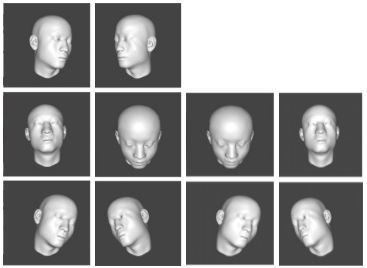
\includegraphics[scale=1]{figheads}
	\caption{Different head poses based from estimated head pose results (Liu, F. et. al., 2015)}
\end{figure}


\begin{table}[!htb]
	\caption{Evaluation of level of Drowsiness}
	\begin{center}
	\begin{tabular}{|c|c|}
		\hline
		\textbf{Level of Drowsiness} & \textbf{Description}                                                                                             \\ \hline
		Awake                        & \begin{tabular}[c]{@{}c@{}}Normal blink rate (0.25 - 0.33 blink/s)\\Normal blink duration (100-400ms)\\Or \\Low blink rate (less than 0.25blink/s) \\Normal blink duration(100-400ms) \end{tabular}         
		\\ \hline
		Low Alertness                & \begin{tabular}[c]{@{}c@{}}Normal blink rate (0.33blink/s - 0.25blink/s)\\Long blink duration(400ms - 1s)\\Or\\Low blink rate (lower than 0.25blink/s)\\Long blink duration(100-400ms) \end{tabular} 
		\\ \hline
		Drowsy                       & \begin{tabular}{@{}c@{}}High blink rate (greater than 0.33blink/s)\\Long blink duration (400ms-1s)\\Or\\Normal blink rate\\Long blink duration (400ms - 1s)\end{tabular} 
                                                                                 
		\\ \hline
		Sleepy                       & \begin{tabular}[c]{@{}c@{}}Low Blink Rate (less than 0.25blink/s)\\Very long Blink Duration (greater than 1s)\end{tabular}
        \\ \hline
		
	\end{tabular}
	\end{center}
	\end{table}
	
\newpage
Using Labview, an algorithm will be made for the evaluation of driver fatigue. It is evaluated into four levels such as Awake, Low Alertness, Drowsy, and Sleeping. Each level of drowsiness will have an indicator and if the driver is evaluated as sleeping or drowsy an alarm will sound off to warn the driver. 

\begin{center}
\begin{figure}[ht]
	\centering
	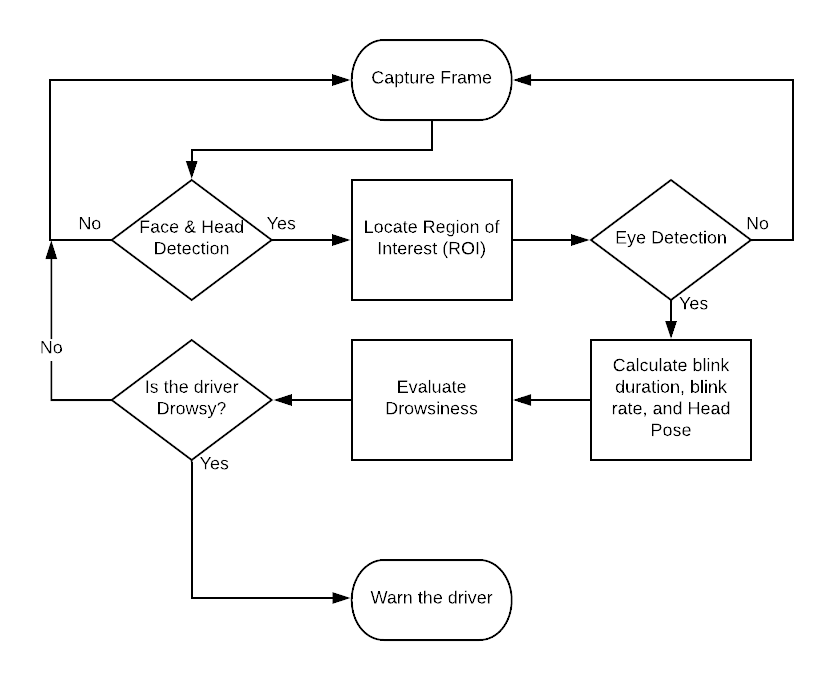
\includegraphics[scale=0.4]{EyeFlowchart}
	\caption{ Evaluation of level of Drowsiness based on blink rate and blink duration}
\end{figure}
\end{center}

\newpage 
The RGB-D camera is continuously taking a video of the face of the driver and frames will be captured. If the face and head is now detected, the edges of the faces will then be taken in order to find the location of the eyes. After eye detection, blink rate, blink duration, and head pose was calculated for evaluation of driver drowsiness. The algorithm to be used for the evaluation of drowsiness will be classifiers. Some examples that can be used as classifiers are machine learning algorithms, fuzzy logic, etc.


\begin{center}
	\begin{figure}[ht]
		\centering
		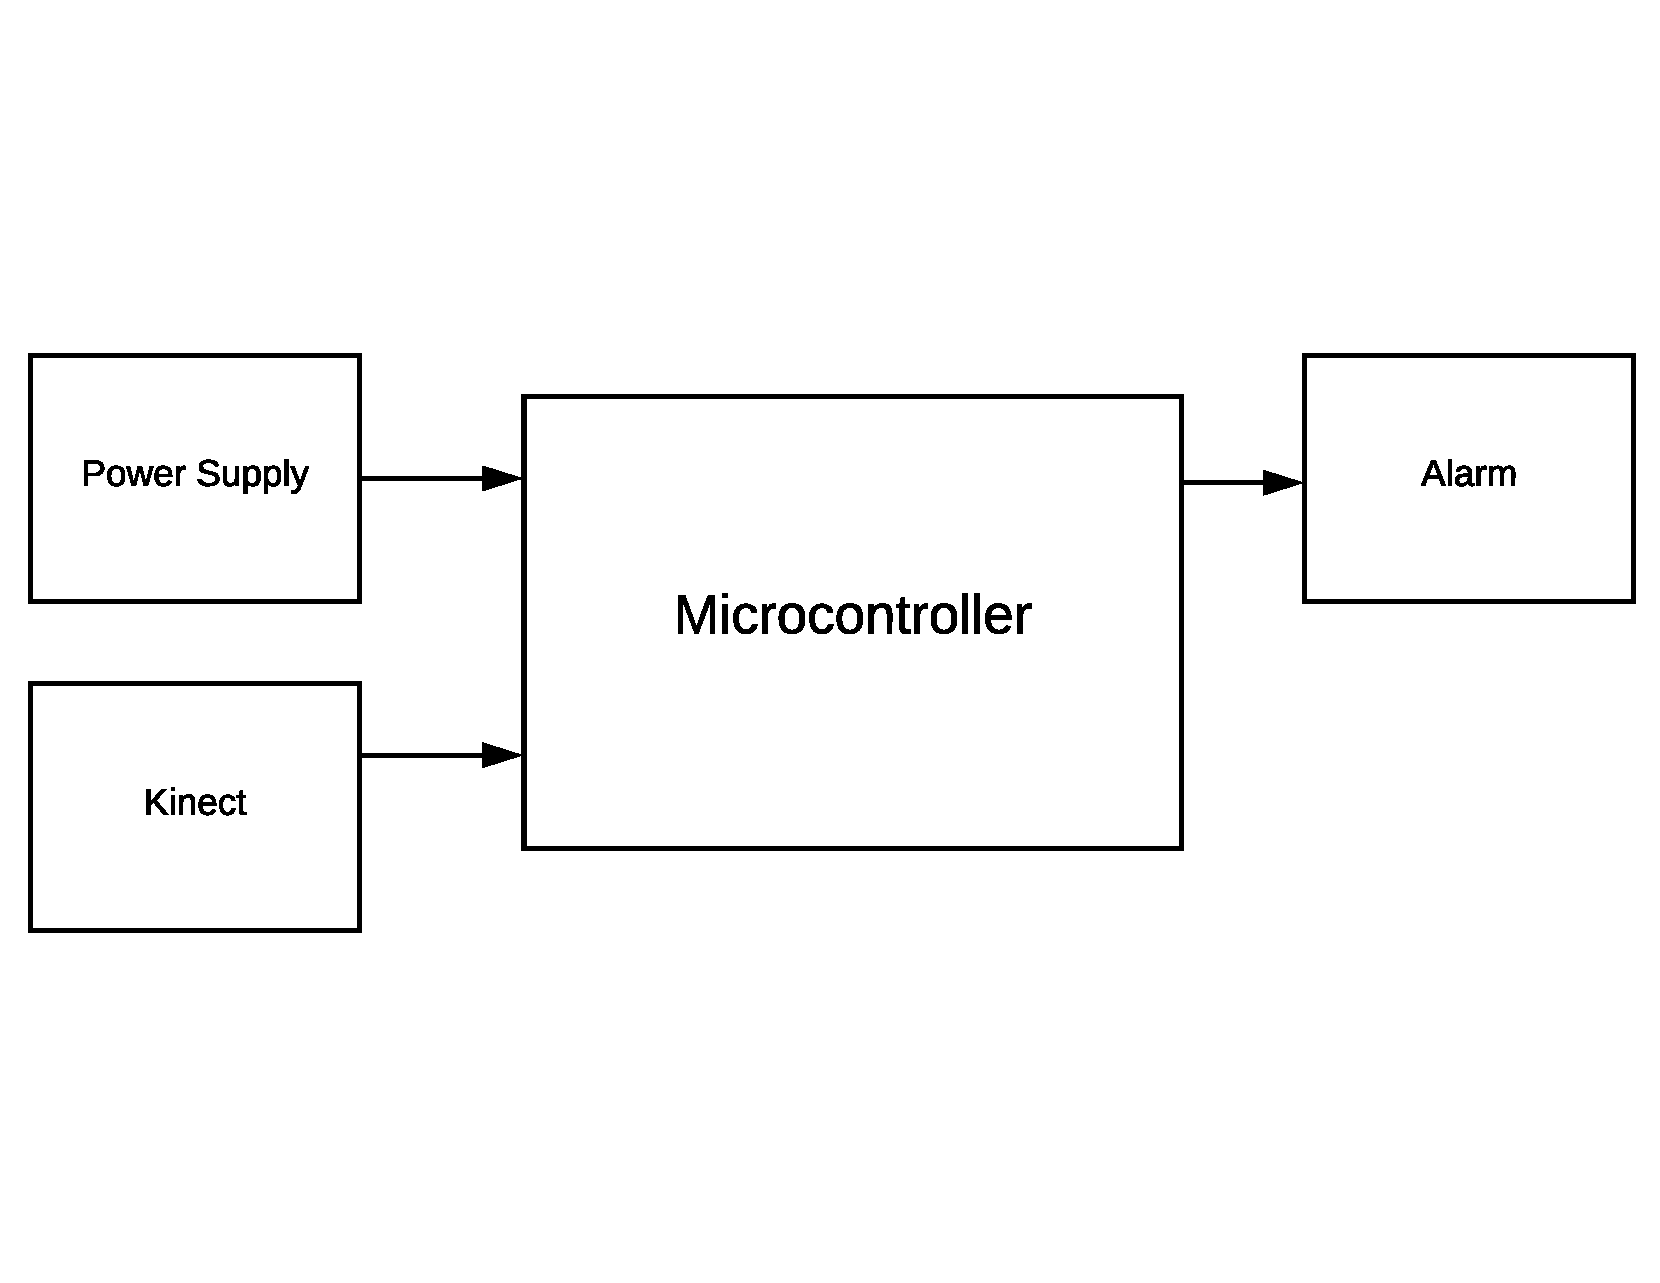
\includegraphics[scale=0.5]{BlockDiagram}
		\caption{Proposed Block Diagram of Driver Monitoring System}
	\end{figure}
\end{center}

\section{Overview}

\subsection{Gantt Chart}
\newpage
The following figures shown below is the individual gantt chart of the researchers:

\begin{figure}[!htb]
	\centering
	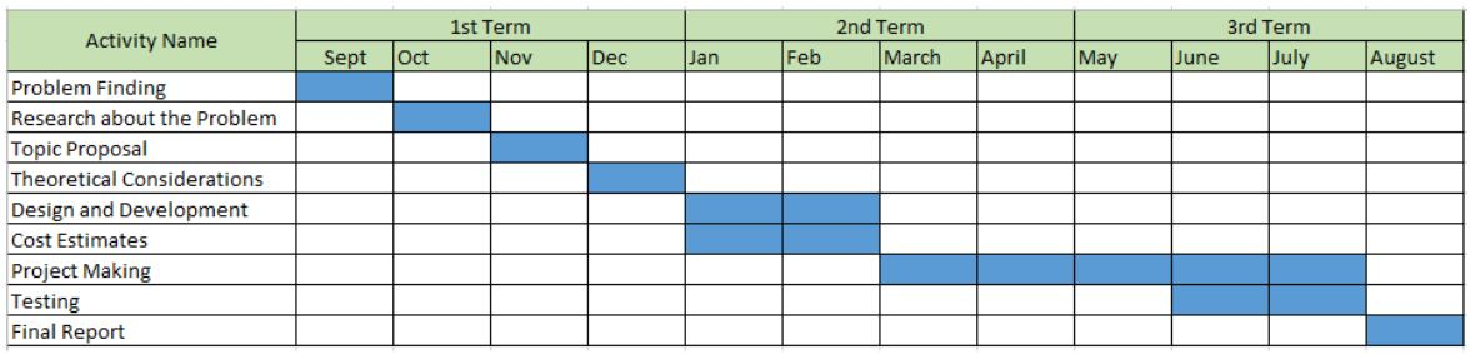
\includegraphics[scale=0.25]{gantt1}
	\caption{Gantt Chart of Guevarra}
\end{figure}
\begin{figure}[!htb]
	\centering
	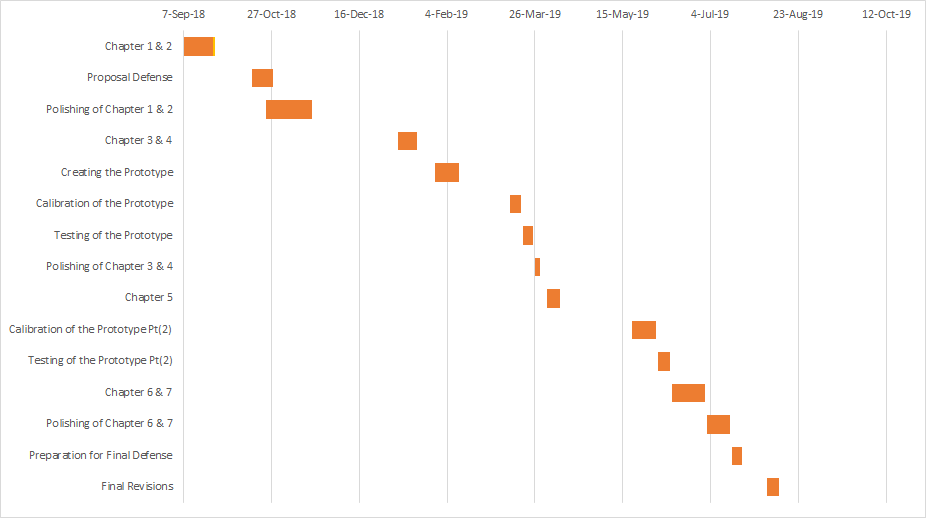
\includegraphics[scale=0.6]{gantt2}
	\caption{Gantt Chart of Hernandez}
\end{figure}
\begin{figure}[!htb]
	\centering
	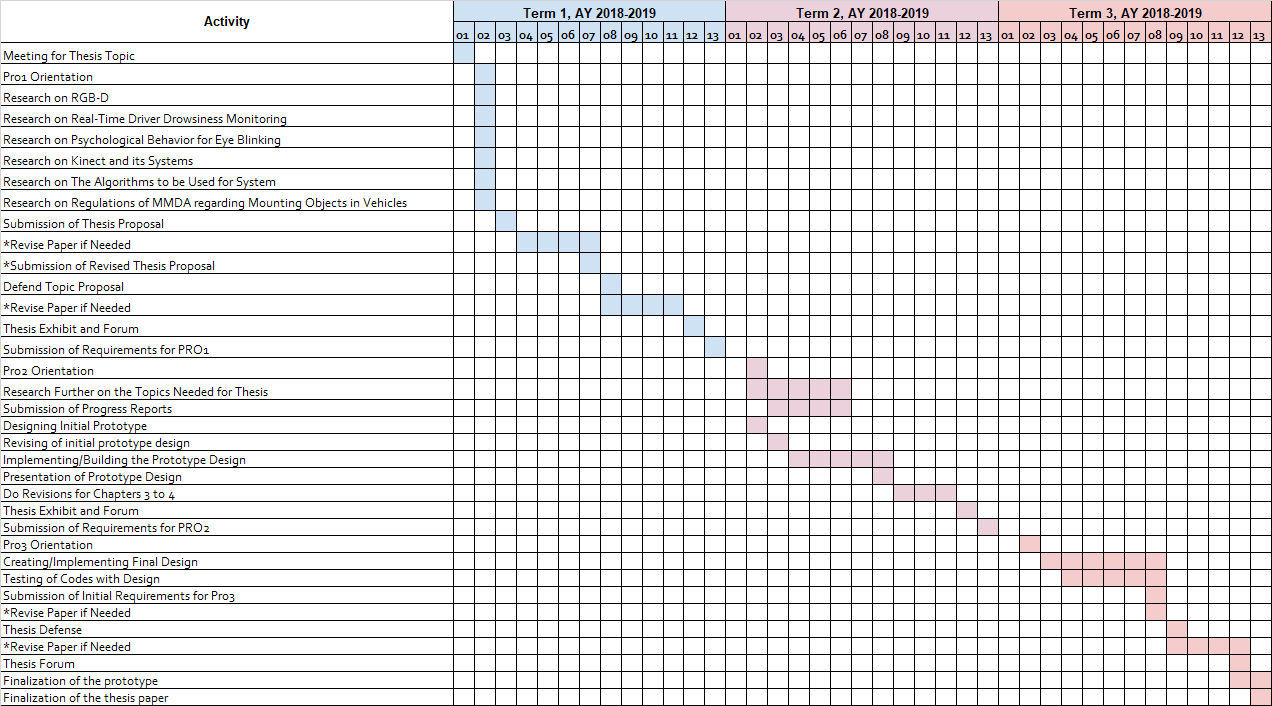
\includegraphics[scale=0.42]{gantt3.png}
	\caption{Gantt Chart of Lagman}
\end{figure}
\begin{figure}[!htb]
	\centering
	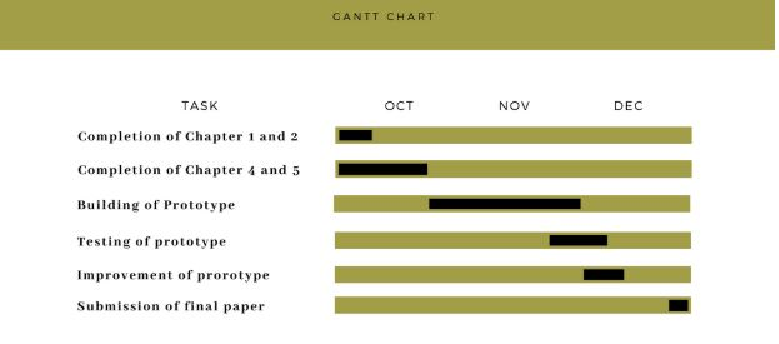
\includegraphics[scale=0.6]{gantt4}
	\caption{Gantt Chart of Villanueva}
\end{figure}
\newpage
\newpage
\subsection{Estimated Work Schedule and Budget}
\begin{table}[!htb]
	\caption{Price List of Materials to be Used}
	\centering
	\begin{tabular}{|c|c|}
		\hline
		Materials & Estimated Price(in PHP) \\
		\hline
		RGB-D Sensor & 10,000-20,000 \\
		\hline
		Microcontroller & 450-2,000 \\
		\hline
		Laptop & Already Available \\
		\hline
		Total Price & 10,450-28,300 \\
		\hline
	\end{tabular}
\end{table}